%%%%%%%%%%%%%%%%%%%%%%%%%%%%%%%%%%%%%%%%%
% Ay 190 - WS2
% Written by Chatarin Wong-u-railertkun
%%%%%%%%%%%%%%%%%%%%%%%%%%%%%%%%%%%%%%%%%

%----------------------------------------------------------------------------------------
%	PACKAGES AND OTHER DOCUMENT CONFIGURATIONS
%----------------------------------------------------------------------------------------

\documentclass[11pt,letterpaper]{article}

% Load some basic packages that are useful to have
% and that should be part of any LaTeX installation.
%

\usepackage{graphicx}     % be able to include figures

\usepackage{xcolor}         % get nice colors

% change default font to Palatino (looks nicer!)
\usepackage[latin1]{inputenc}
\usepackage{mathpazo}
\usepackage[T1]{fontenc}

% load some useful math symbols/fonts
\usepackage{latexsym,amsfonts,amsmath,amssymb}
\usepackage{subcaption}

% comfort package to easily set margins
\usepackage[top=1in, bottom=1in, left=1in, right=1in]{geometry}

% control some spacings
%
% spacing after a paragraph
\setlength{\parskip}{.15cm}
% indentation at the top of a new paragraph
\setlength{\parindent}{0.0cm}

\usepackage{courier}


%----------------------------------------------------------------------------------------
%	TITLE
%----------------------------------------------------------------------------------------

\begin{document}

\begin{center}
\Large
Ay190 -- Worksheet 16 \\    %%%%%% DON'T FORGET TO CHANGE THE WORK SHEET NUMBER
Chatarin (Mee) Wong-u-railertkun\\
Date: \today
\end{center}

\section{Finite Volume Hydro Code}

\subsection{Structure}

For every loop, we calculate new time step. Then, using RK2 to calculate the new data with the helper function to calculate RHS. Apply boundary conditions into the RK2 also. Same as the diagram in the lecture note, at the end of RK2, we use the helper function \texttt{con2prim}. The \texttt{mydata} Class stores all values, which are easier to access and keep track. 

\subsection{Evolution}
	
\begin{figure}[h!]
	\centering
	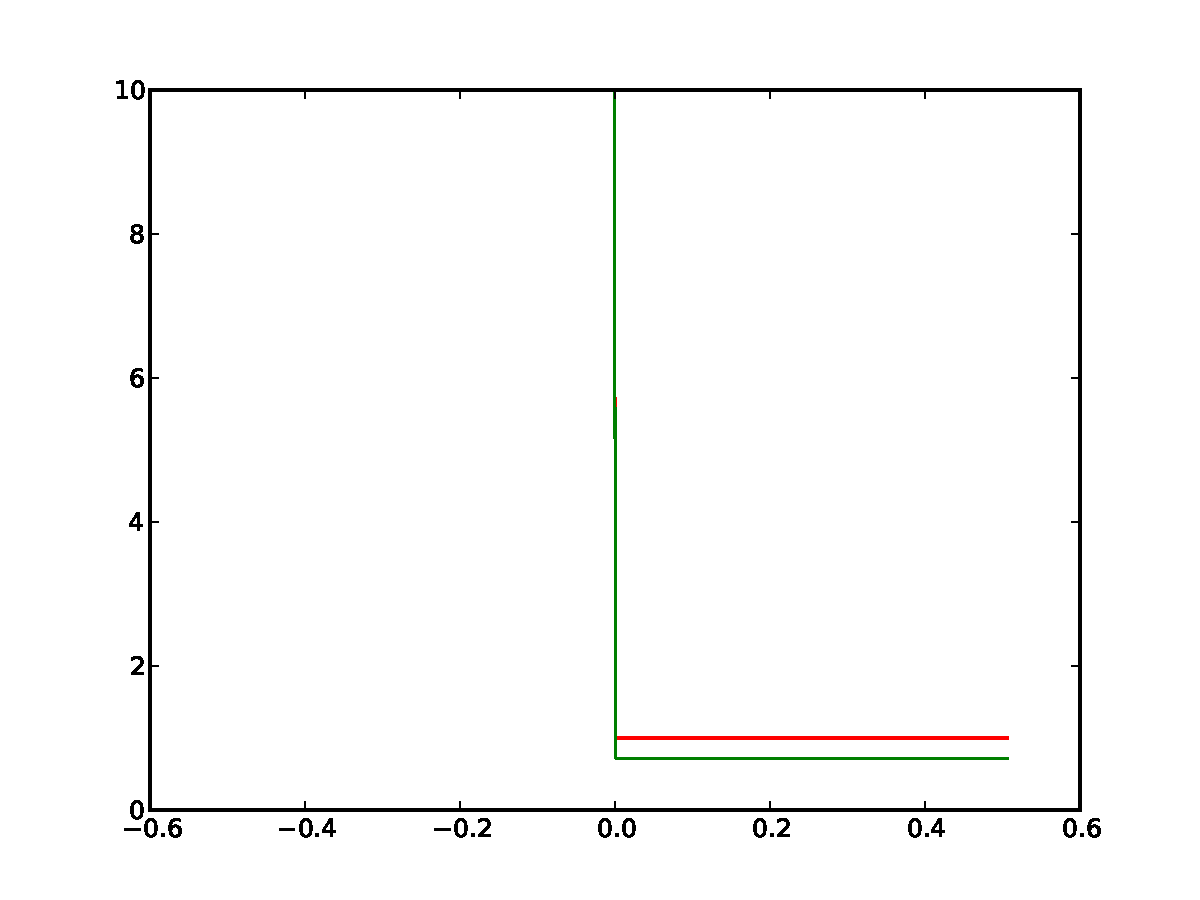
\includegraphics[width=0.45\textwidth]{plot1}
	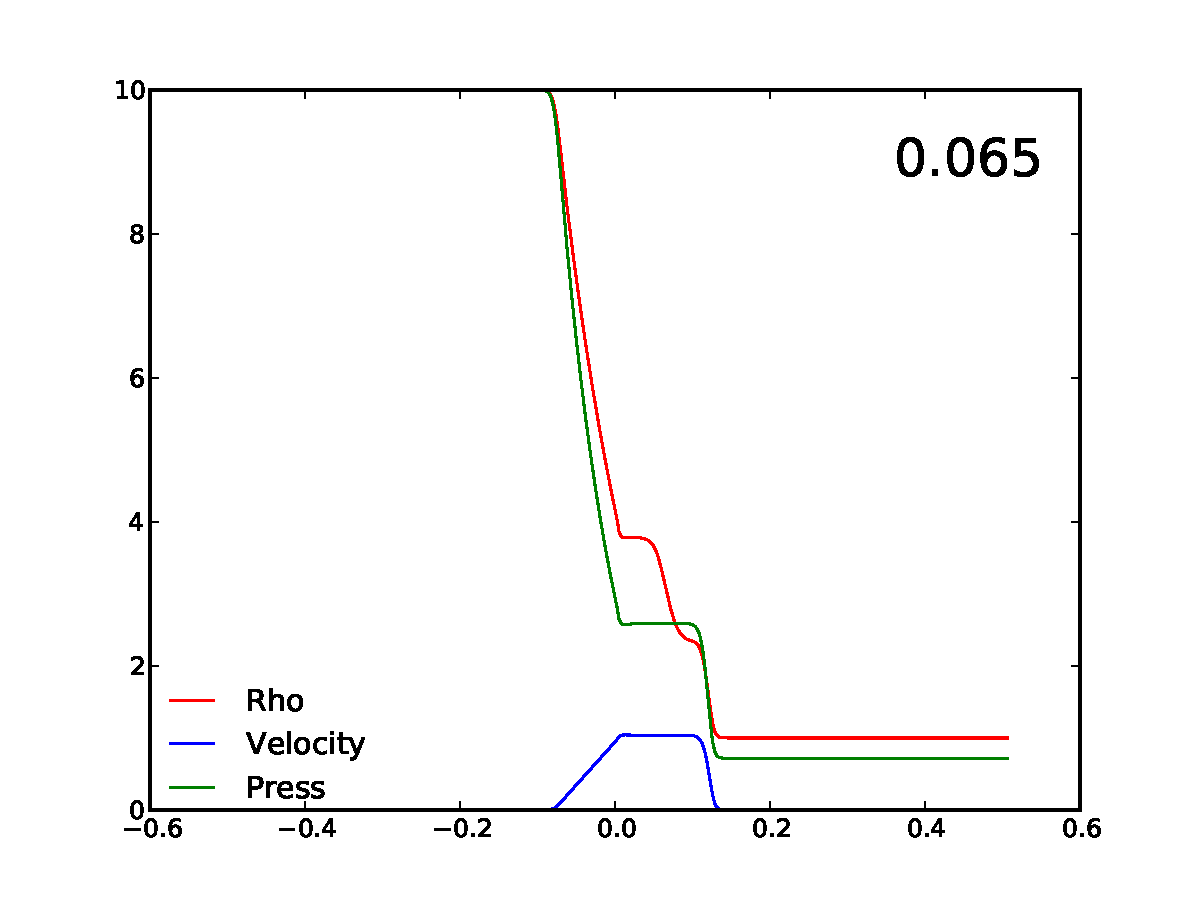
\includegraphics[width=0.45\textwidth]{plot2}
\end{figure}
\begin{figure}[h!]
	\centering
	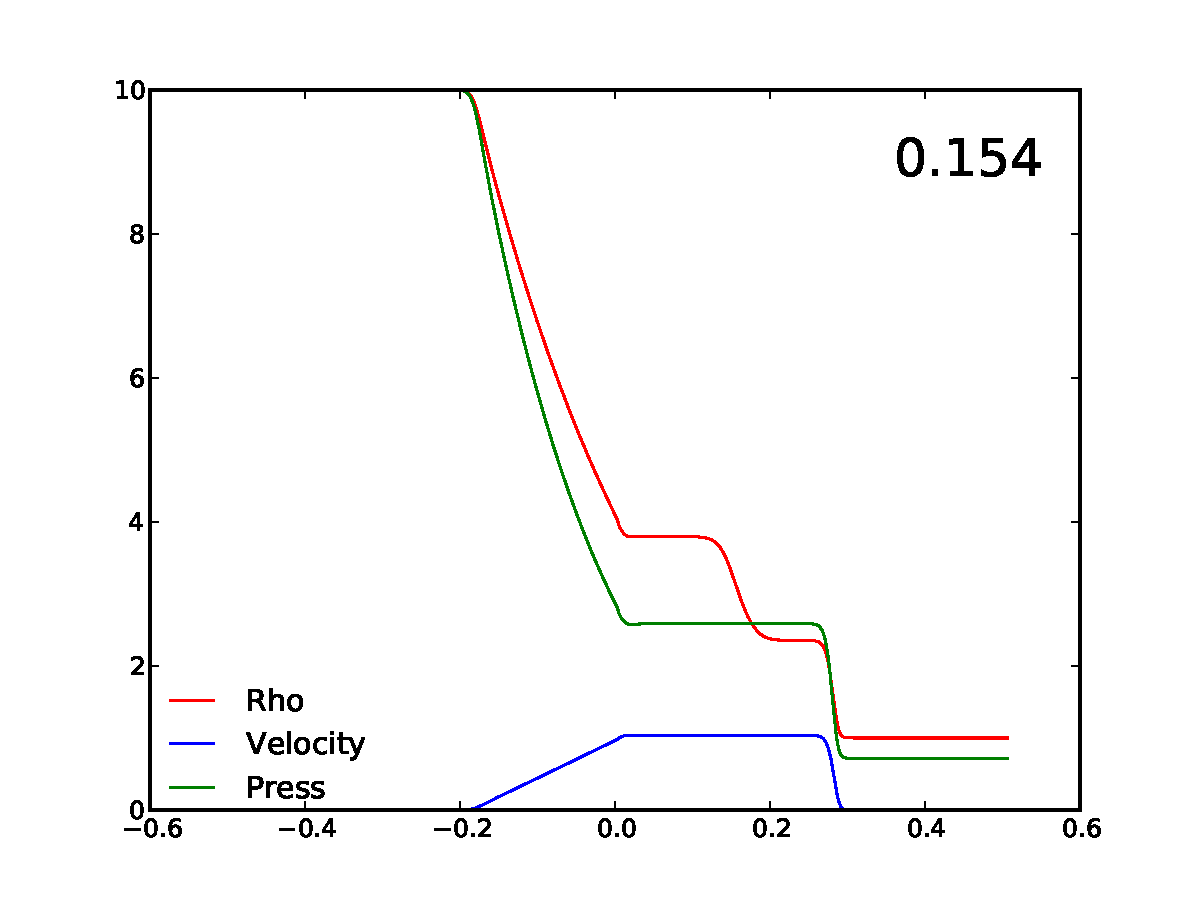
\includegraphics[width=0.45\textwidth]{plot3}
	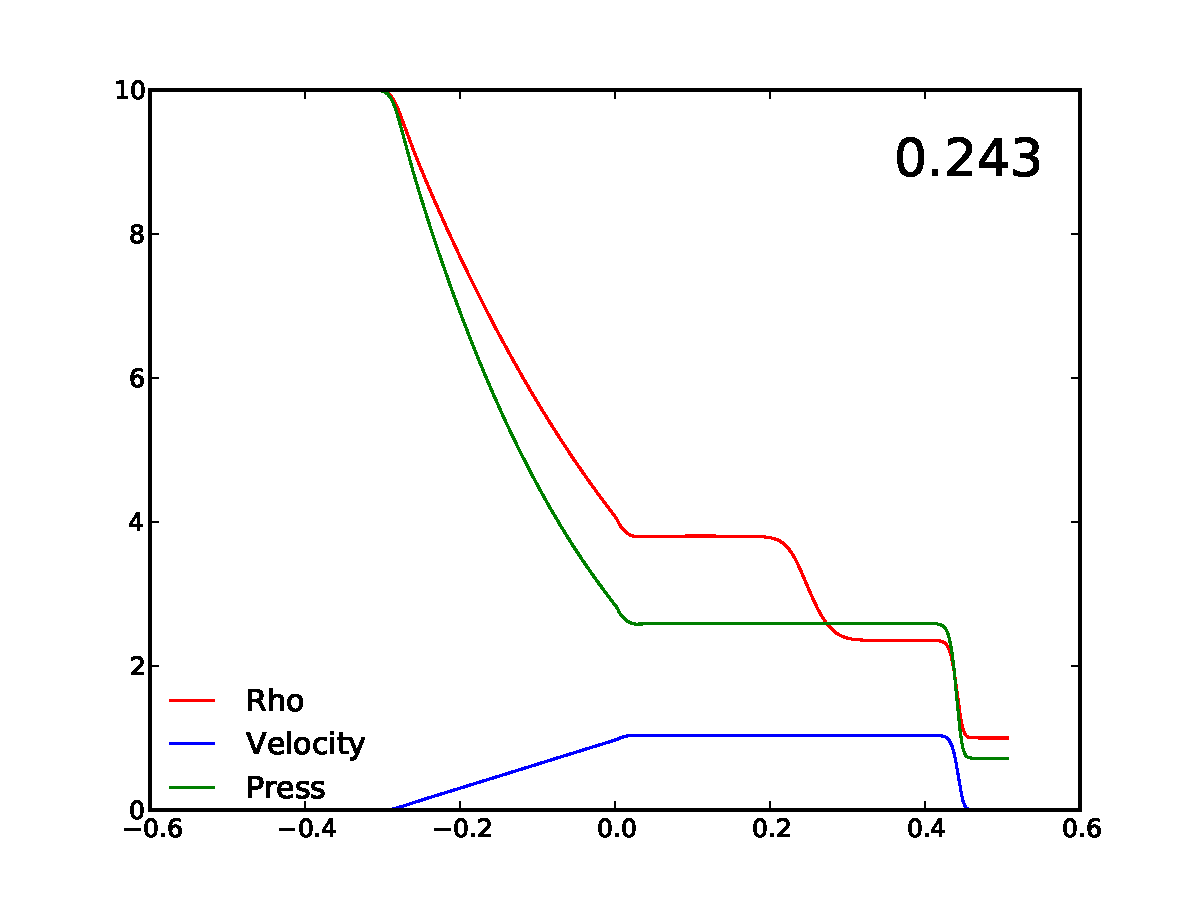
\includegraphics[width=0.45\textwidth]{plot4}
\end{figure}
\begin{figure}[h!]
	\centering
	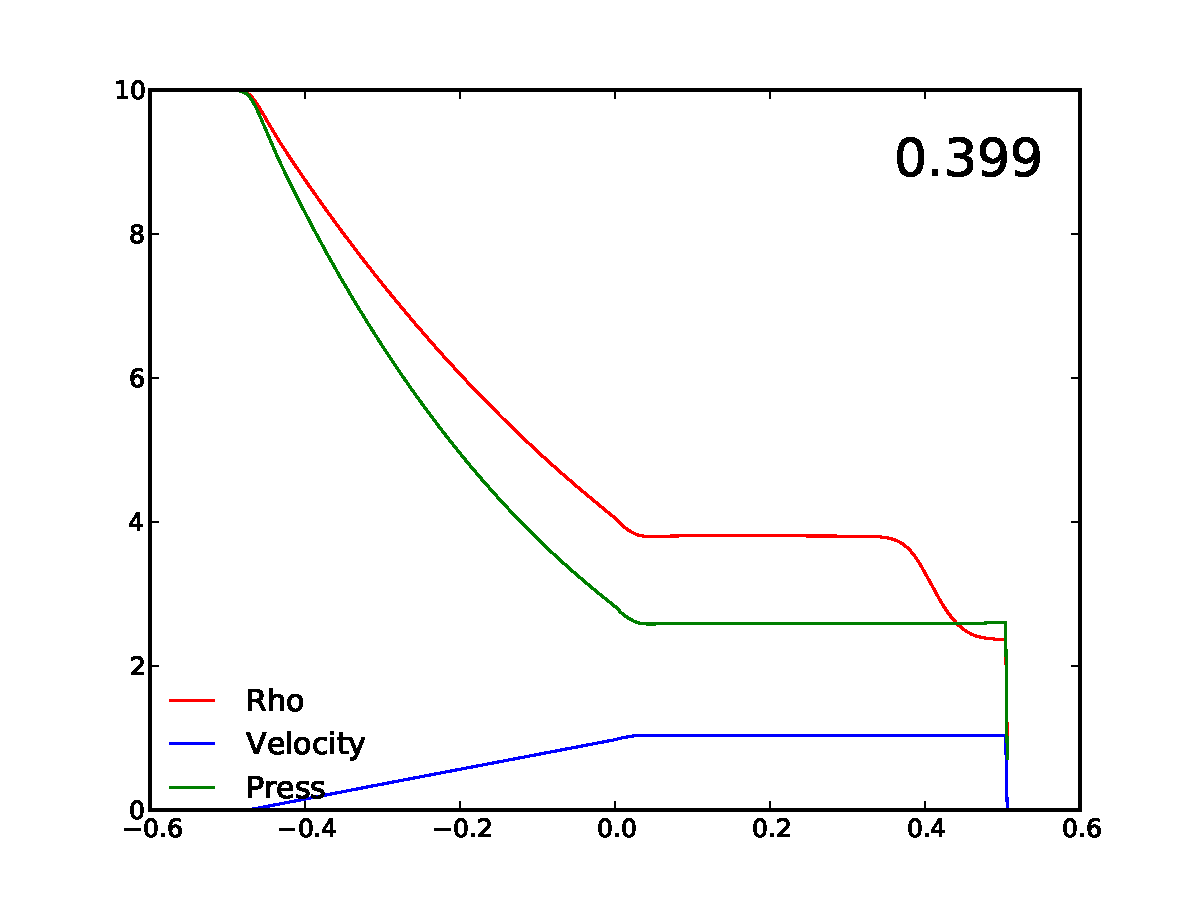
\includegraphics[width=0.45\textwidth]{plot5}
\end{figure}	
\end{document}

